\documentclass[twocolumn]{aastex631}
\makeatletter
\def\ps@plain{%
  \let\@mkboth\@gobbletwo
  \def\@oddhead{}%
  \def\@evenhead{}%
  \def\@oddfoot{\hfil\thepage\hfil}%
  \def\@evenfoot{\hfil\thepage\hfil}%
}
\let\ps@headings\ps@plain
\let\ps@myheadings\ps@plain
\let\ps@article\ps@plain
\let\ps@aas@headings\ps@plain
\def\@journalinfo{}
\def\@slugcomment{}
\def\frontmatter@title@above{}
\makeatother
\pagestyle{plain}
\usepackage{amsmath}
\usepackage{graphicx}
\usepackage{booktabs}
\usepackage{array}
\usepackage{microtype}
\newcommand{\kms}{km\,s$^{-1}$}
\renewcommand{\bibfont}{\tiny}

\begin{document}
\pagestyle{plain}
\sloppy
\hbadness=10000
\hyphenpenalty=10000
\exhyphenpenalty=10000

\title{Empirical Response Exponents and Geometric-Medium Information in Galaxy Rotation Curves}
\correspondingauthor{Mohammed Messaoudene}
\email{mohammed.messaoudene@univ-temouchent.edu.dz}
\author[0009-0007-4665-2548]{Mohammed Messaoudene}
\affiliation{Faculty of Sciences, Belhadj Bouchaib University of Ain Temouchent, Route of Sidi Bel Abbes, BP 284, 46000 Ain Temouchent, Algeria}

\begin{abstract}
Galaxy rotation curves measure a single radial acceleration, but that scalar need not come from a single physical channel.  I use a channel-aware response framework in which the Newtonian baryonic source and the inferred dark or geometric response are distinct contributions projected onto the observed rotation curve.  The parent form introduces an internal alignment $\kappa=\cos\theta_{\rm int}$ and a response amplitude $g_\chi=A_\chi g_N^p$; the empirical tests use the projected closure $g_{\rm tot}=g_N+A_{\rm eff}g_N^p$.  This response-exponent view is compared with a fixed Geometric-Medium Response (GMR) prescription tested on SPARC.  GMR contains a square-root response core, although a pure square-root control remains slightly better on the main SPARC equal-weight RMSE benchmark.  The GMR construction is nevertheless useful: it is competitive with baryons-only, MOND, and reduced NFW in that aggregate metric, its cumulative state improves over a local-state ablation, and its failures identify low-density dwarf and low-surface-brightness systems as the principal tension.  Direct LSB mass models favor a fixed $p\simeq0.298$ comparison branch, whereas LITTLE THINGS proxy and validated vector-recovered subsets lean toward $p=0.5$ without decisive significance.  These results do not define a universal exponent and do not solve the dark-sector problem.  They instead show that the projected response branch is sensitive to data set, metric, and baryonic modeling, and that free-exponent fits with propagated uncertainties are the next necessary test.
\end{abstract}
\keywords{Galaxy rotation curves (619) --- Disk galaxies (391) --- Dwarf galaxies (416) --- Low surface brightness galaxies (940) --- Dark matter (353) --- Astrostatistics (1882)}

\section{Introduction}
The discrepancy between observed galaxy rotation curves and the acceleration expected from visible matter is one of the clearest empirical entry points into the dark-sector problem \citep{Rubin1970,Rubin1980,Bosma1981,Begeman1991,SofueRubin2001}.  SPARC placed that question on a homogeneous footing by combining resolved rotation curves with infrared photometry and baryonic mass models for 175 disk galaxies \citep{Lelli2016SPARC}.  The same data set also sharpened the radial-acceleration relation and baryonic Tully-Fisher relation \citep{McGaugh2016RAR,Lelli2017BTFR,McGaugh2012}.  A useful phenomenological question is therefore not only which model fits, but what kind of baryonic information a missing-response model is actually using.

I therefore treat the exponent in a response law,
\begin{equation}
g_{\rm resp}=A g_N^p ,
\end{equation}
as a measured property of the projected response channel.  The exponent is not introduced as a new law by itself.  It is a concise way to ask how the inferred non-baryonic acceleration scales with the baryonic source once the metric, calibration, and data provenance have been fixed.

\section{Channel-aware response}
The organizing idea is that two quantities can both have the dimensions of acceleration without belonging to the same physical channel.  Let $g_N$ denote the Newtonian baryonic source amplitude and $g_\chi$ the inferred response amplitude.  In an internal response space,
\begin{equation}
{\bf G}_{\rm tot}=g_N{\bf e}_b+g_\chi{\bf e}_\chi,
\qquad
{\bf e}_b\cdot{\bf e}_\chi=\kappa=\cos\theta_{\rm int} .
\end{equation}
The observable norm is then
\begin{equation}
g_{\rm tot}^2=g_N^2+g_\chi^2+2\kappa g_Ng_\chi .
\end{equation}
With
\begin{equation}
g_\chi=A_\chi g_N^p ,
\end{equation}
one obtains
\begin{equation}
g_{\rm tot}=
\left[g_N^2+A_\chi^2g_N^{2p}+
2\kappa A_\chi g_N^{p+1}\right]^{1/2} .
\end{equation}
The tests below use the effective radial projection
\begin{equation}
g_{\rm tot}=g_N+A_{\rm eff}g_N^p .
\end{equation}
For $g_\chi/g_N\ll1$ and approximately constant $\kappa$, Eq.~(5) expands as $g_{\rm tot}=g_N+\kappa A_\chi g_N^p+\frac{1}{2}(1-\kappa^2)A_\chi^2g_N^{2p-1}+\cdots$.  Thus $A_{\rm eff}$ is not assumed to be $A_\chi$; it equals $\kappa A_\chi$ only at leading order in this restricted projection.  If $\kappa$ or $A_\chi$ varies with environment, the fitted $p$ is an effective response exponent.  In the fits below, $A_{\rm eff}$ is only the amplitude of the projected scalar closure.  The analysis does not separate $\kappa$ from $A_\chi$, and does not infer either quantity independently.  The variables $\kappa$ and $\theta_{\rm int}$ remain parent-geometry variables.

\begin{figure}[t]
\centering
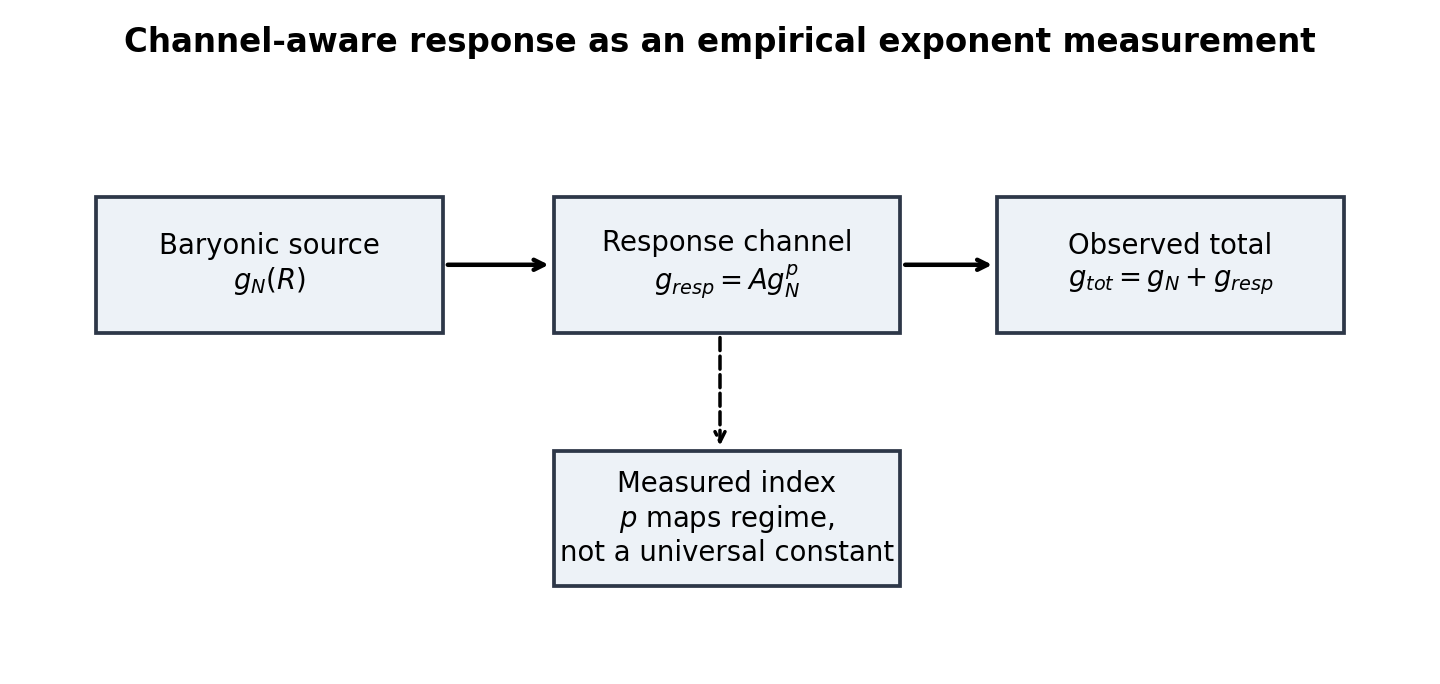
\includegraphics[width=0.92\columnwidth]{figures/R124_FIG1_conceptual_response_channel.png}
\caption{Schematic hierarchy of the channel-aware response idea.  The scalar law tested here is the radial projection of a response-channel model, not the full theory.}
\end{figure}

\section{The fixed GMR prescription}
The fixed GMR prescription turns several baryonic-geometry quantities into a response operator.  It uses local tidal and curvature information.  Here $T_{ij}=\partial_i\partial_j\phi_B$ is the baryonic tidal tensor and $\|T\|$ is its Frobenius norm.  The scalar $|\nabla^2\phi_B|$ is the magnitude of the baryonic Laplacian; the small floor $\epsilon_A$ carries the same denominator units.  With this convention $A_B$ is a dimensionless local anisotropy measure rather than a new acceleration scale:
\begin{equation}
A_B(R)=\frac{\|T(R)\|}{|\nabla^2\phi_B(R)|+\epsilon_A},
\end{equation}
\begin{equation}
C_B(R)=
\frac{\ell_*|\nabla^2\phi_B(R)|}
{\left[(\partial_R\phi_B)^2+A_*^2+\epsilon_C\right]^{1/2}},
\end{equation}
where $\epsilon_C$ has the dimensions of the squared radial-field term in the bracket.  The bounded local tracer is
\begin{equation}
\nu_B(R)=\frac{A_B(R)+C_B(R)}{1+A_B(R)+C_B(R)} .
\end{equation}
Its non-local state is cumulative:
\begin{equation}
Q_{\rm enc}(R_i)=\sum_{j\le i}\nu_B(R_j)\Delta R_j,
\end{equation}
The radial samples are sorted by increasing $R_i$ before this cumulative state is evaluated; $\Delta R_j$ is the adjacent radial spacing in that ordered profile.  The implementation tested here treats this as a first-order cumulative radial feature, not as a high-order quadrature estimate of a unique continuum integral.  The comparison therefore tests this specific ordered feature and does not claim invariance under alternative radial integration rules.
\begin{equation}
S_\Psi(R_i)=
\frac{Q_{\rm enc}(R_i)}{Q_*+Q_{\rm enc}(R_i)} .
\end{equation}
The response angle and suppression factor are
\begin{equation}
\alpha_B(R_i)=\arctan
\left[
\frac{A_B(R_i)+\eta_S S_\Psi(R_i)}{1+C_B(R_i)}
\right],
\end{equation}
\begin{equation}
S_{\rm rad}(R_i)=
\left[1+\lambda_s\nu_B(R_i)C_B(R_i)\right]^{-1} .
\end{equation}
The response acceleration is
\begin{equation}
g_\chi^{\rm GMR}(R_i)=
\mathcal A_{\rm GMR}\sin\alpha_B(R_i)
\sqrt{g_N(R_i)}S_{\rm rad}(R_i).
\end{equation}
Thus the prescription contains a square-root core but is not identical to a pure square-root law: the factor $\sin\alpha_B S_{\rm rad}$ carries the tested geometric information.  The grid used here has $\mathcal A_{\rm GMR}=1.39458\times10^{-5}$ and $\lambda_s=10.0$.  In the rotation-curve convention used for the calculations, accelerations are stored as $g=V^2/R$ with $V$ in km\,s$^{-1}$ and $R$ in kpc; hence $g$ has units km$^2$\,s$^{-2}$\,kpc$^{-1}$ and $\mathcal A_{\rm GMR}$ has units km\,s$^{-1}$\,kpc$^{-1/2}$.  These values are kept fixed in the external response-exponent comparisons.

\begin{figure}[t]
\centering
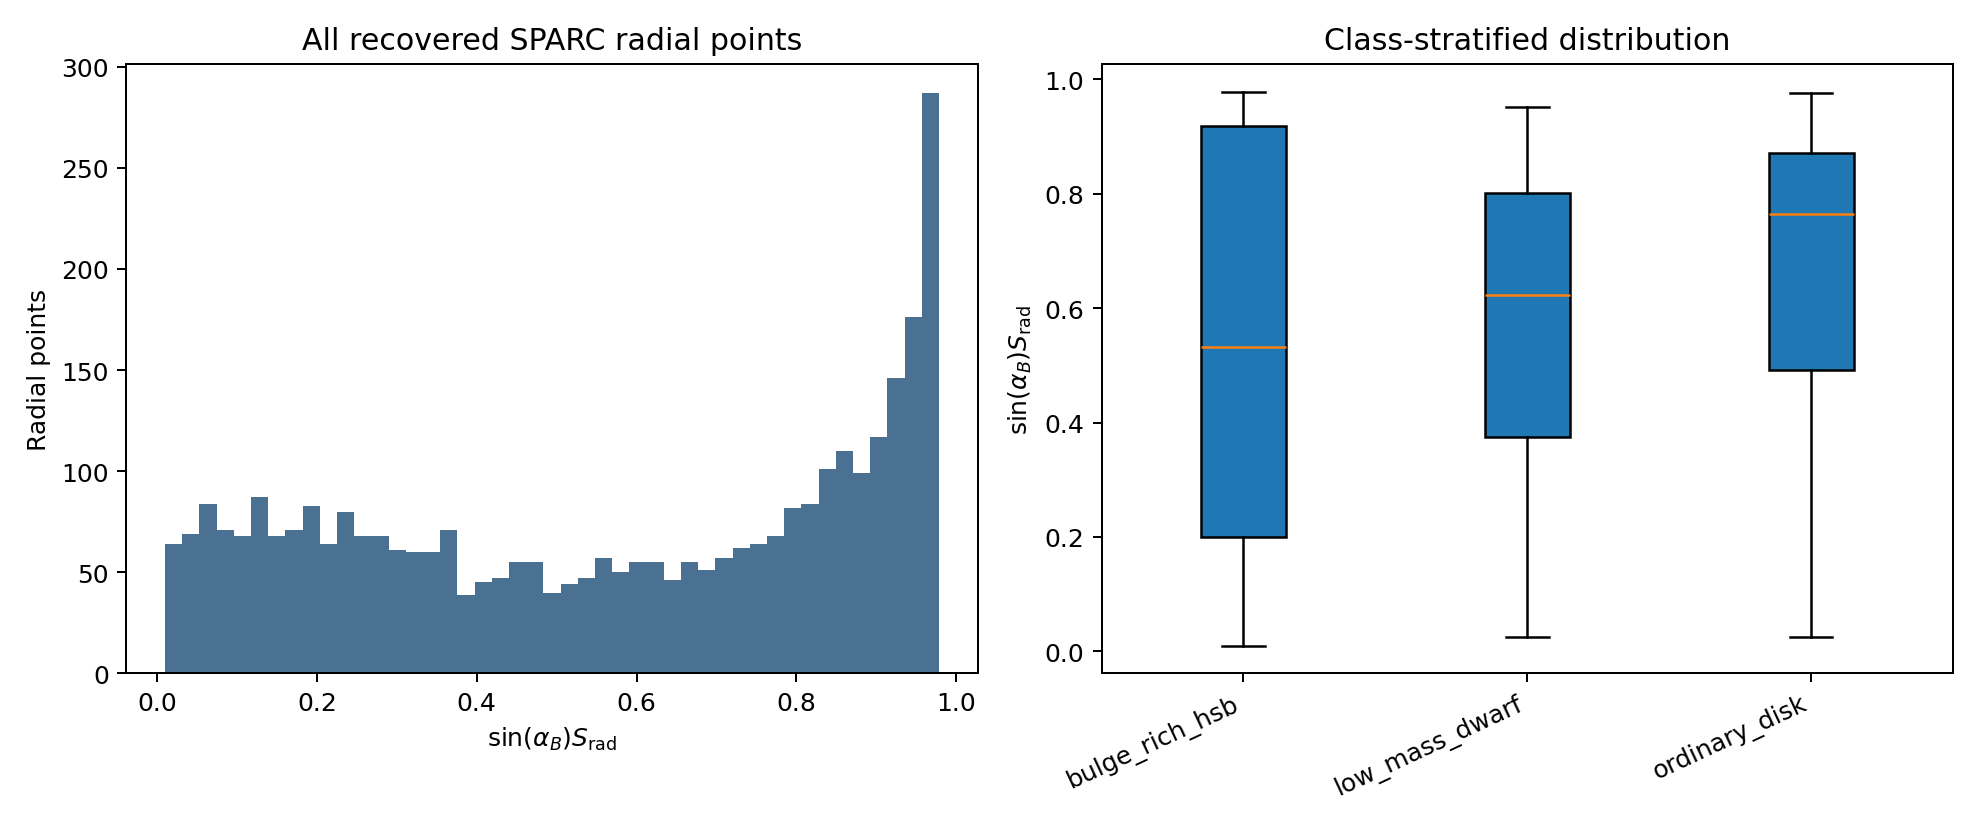
\includegraphics[width=0.92\columnwidth]{figures/V55_FIG6_sin_alpha_Srad_diagnostic.png}
\caption{The GMR modulation factor is not constant.  The fixed prescription contains a square-root core but also tests whether baryonic invariants add predictive information.}
\end{figure}

\section{Data sets and evidence tiers}
The analysis keeps four evidence tiers separate.  SPARC is the main internal benchmark.  A public low-surface-brightness sample provides a small but direct component test with explicit gas, disk, and bulge velocities \citep{deBlok2001}.  LITTLE THINGS is used in two more cautious ways: as a proxy based on public total and dark-matter curves, and as a vector-recovered component subset from published mass-model figures \citep{Hunter2012,Oh2015}.

\begin{table}[t]
\centering
\scriptsize
\begin{tabular}{@{}llll@{}}
\toprule
Tier & Data & Input & Role\\
\midrule
Internal & SPARC & mass models & main\\
Direct & LSB & components & external\\
Proxy & LT & $V_{\rm tot}^2-V_{\rm DM}^2$ & stress test\\
Vector & LT & vector-recovered & appendix caveat\\
\bottomrule
\end{tabular}
\caption{Evidence tiers.  Proxy/vector quantities are not official component tables.}
\end{table}

\subsection{Response-exponent estimation}
For a fixed exponent $p$, the projected scalar control is evaluated as $g_{\rm model}=g_N+A_p g_N^p$ and converted to a circular-speed prediction at each tabulated radius.  The displayed comparisons hold two branches fixed: SQRT uses $p=0.5$, while FREEP uses $p\simeq0.298$.  The latter value comes from the internal OMEGA/SPARC calibration track, where a one-parameter power-law family was scanned under the equal-weight galaxy RMSE objective after fitting the amplitude for each fixed exponent.  Here it serves only as a comparison branch.  It is not re-estimated for each external sample, and no independent physical constant is assigned to it.  Unless a table states otherwise, the objective is the equal-weight galaxy RMSE,
\begin{equation}
{\rm RMSE}_{\rm EW}=\left[\frac{1}{N_{\rm gal}}\sum_g {\rm RMSE}_g^2\right]^{1/2},
\end{equation}
with ${\rm RMSE}_g$ computed from the radial velocity residuals of galaxy $g$.  Observation-weighted RMSE is reported separately where available.  The external comparison table gives fixed-branch tests rather than new per-galaxy free-$p$ fits.  In particular, the phrase ``the $p\simeq0.298$ branch'' denotes a fixed model-comparison branch, not an independent measurement of $p=0.298$ in every data set.

\section{SPARC benchmark}
On the full SPARC sample, the square-root control has an equal-weight RMSE of 40.241 \kms, while fixed GMR gives 40.554 \kms.  On the non-calibration complement, the corresponding values are 41.329 and 41.870 \kms.  The tested GMR invariants therefore do not improve the main equal-weight benchmark beyond the simpler square-root response.

\begin{table}[t]
\centering
\scriptsize
\begin{tabular}{llrrr}
\toprule
Sample & Model & EW & Median & Win\\
\midrule
full & GMR & 40.554 & 16.167 & --\\
full & Baryons & 69.316 & 42.879 & 0.886\\
full & MOND & 44.907 & 28.160 & 0.726\\
full & NFW & 46.613 & 8.401 & 0.320\\
full & ISO & 20.316 & 4.919 & 0.074\\
full & Burkert & 25.862 & 5.646 & 0.086\\
held-out & GMR & 41.870 & 16.033 & --\\
held-out & Baryons & 71.026 & 42.879 & 0.874\\
held-out & MOND & 45.366 & 28.352 & 0.715\\
held-out & NFW & 48.450 & 9.307 & 0.338\\
held-out & ISO & 20.869 & 4.770 & 0.079\\
held-out & Burkert & 27.081 & 5.522 & 0.093\\
\bottomrule
\end{tabular}
\caption{SPARC metrics in \kms.  Win is the GMR win rate against the listed comparator.  Cored halo baselines remain stronger empirical fits overall.}
\end{table}

These numbers resist a simple success-or-failure reading.  In the equal-weight aggregate alone, the fixed GMR prescription has lower RMSE than baryons-only, MOND, and reduced NFW.  Galaxy by galaxy, however, reduced NFW keeps the smaller median residual and higher win rate, while reduced ISO and Burkert remain stronger empirical halo prescriptions overall.  Observation-weighted scoring also changes the ordering: GMR has a full-sample $N_{\rm obs}$-weighted RMSE of 57.334 \kms, whereas MOND gives 52.224 \kms.  The response prescription is therefore best viewed as a structured constraint.  The tabulated RMSE values are point estimates; a complete set of per-model galaxy-bootstrap intervals is not included here.

\begin{figure}[t]
\centering
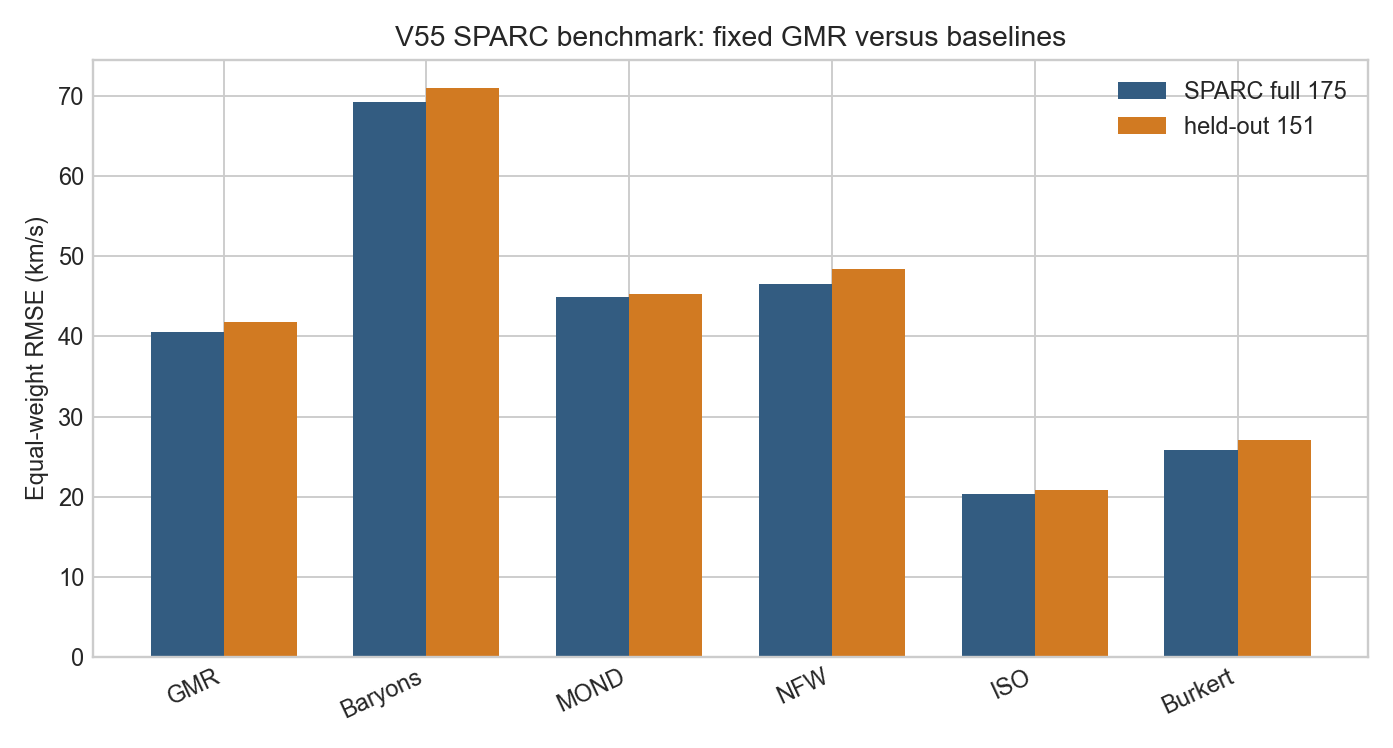
\includegraphics[width=0.92\columnwidth]{figures/R133_FIG_SPARC_AGGREGATE_RMSE.png}
\caption{SPARC aggregate comparison.  The fixed response has non-trivial aggregate behavior, but it does not beat SQRT or the cored halo baselines.}
\end{figure}

\subsection{Ablations and leverage}
The cumulative state variable matters within the GMR family.  Replacing it by a local state gives 47.683 \kms\ on the full sample and 49.398 \kms\ on the held-out subset, substantially worse than the cumulative prescription.  This does not overturn the square-root comparison, but it shows that the cumulative term carries measurable information.

The SPARC aggregate is also leverage-sensitive.  Some large residual improvements occur in a finite set of galaxies, while reduced NFW wins for the majority of individual systems.  For that reason the analysis reports aggregate RMSE, median residual, win rates, observation-weighted metrics, and class stress together.  In the class-stress table, the GMR-over-NFW win fractions are 41/77 for bulge-rich high-surface-brightness systems (0.532; Wilson 95\% interval 0.422--0.640), 11/81 for low-mass dwarfs (0.136; 0.078--0.227), and 4/17 for ordinary disks (0.235; 0.096--0.473).

\begin{figure}[t]
\centering
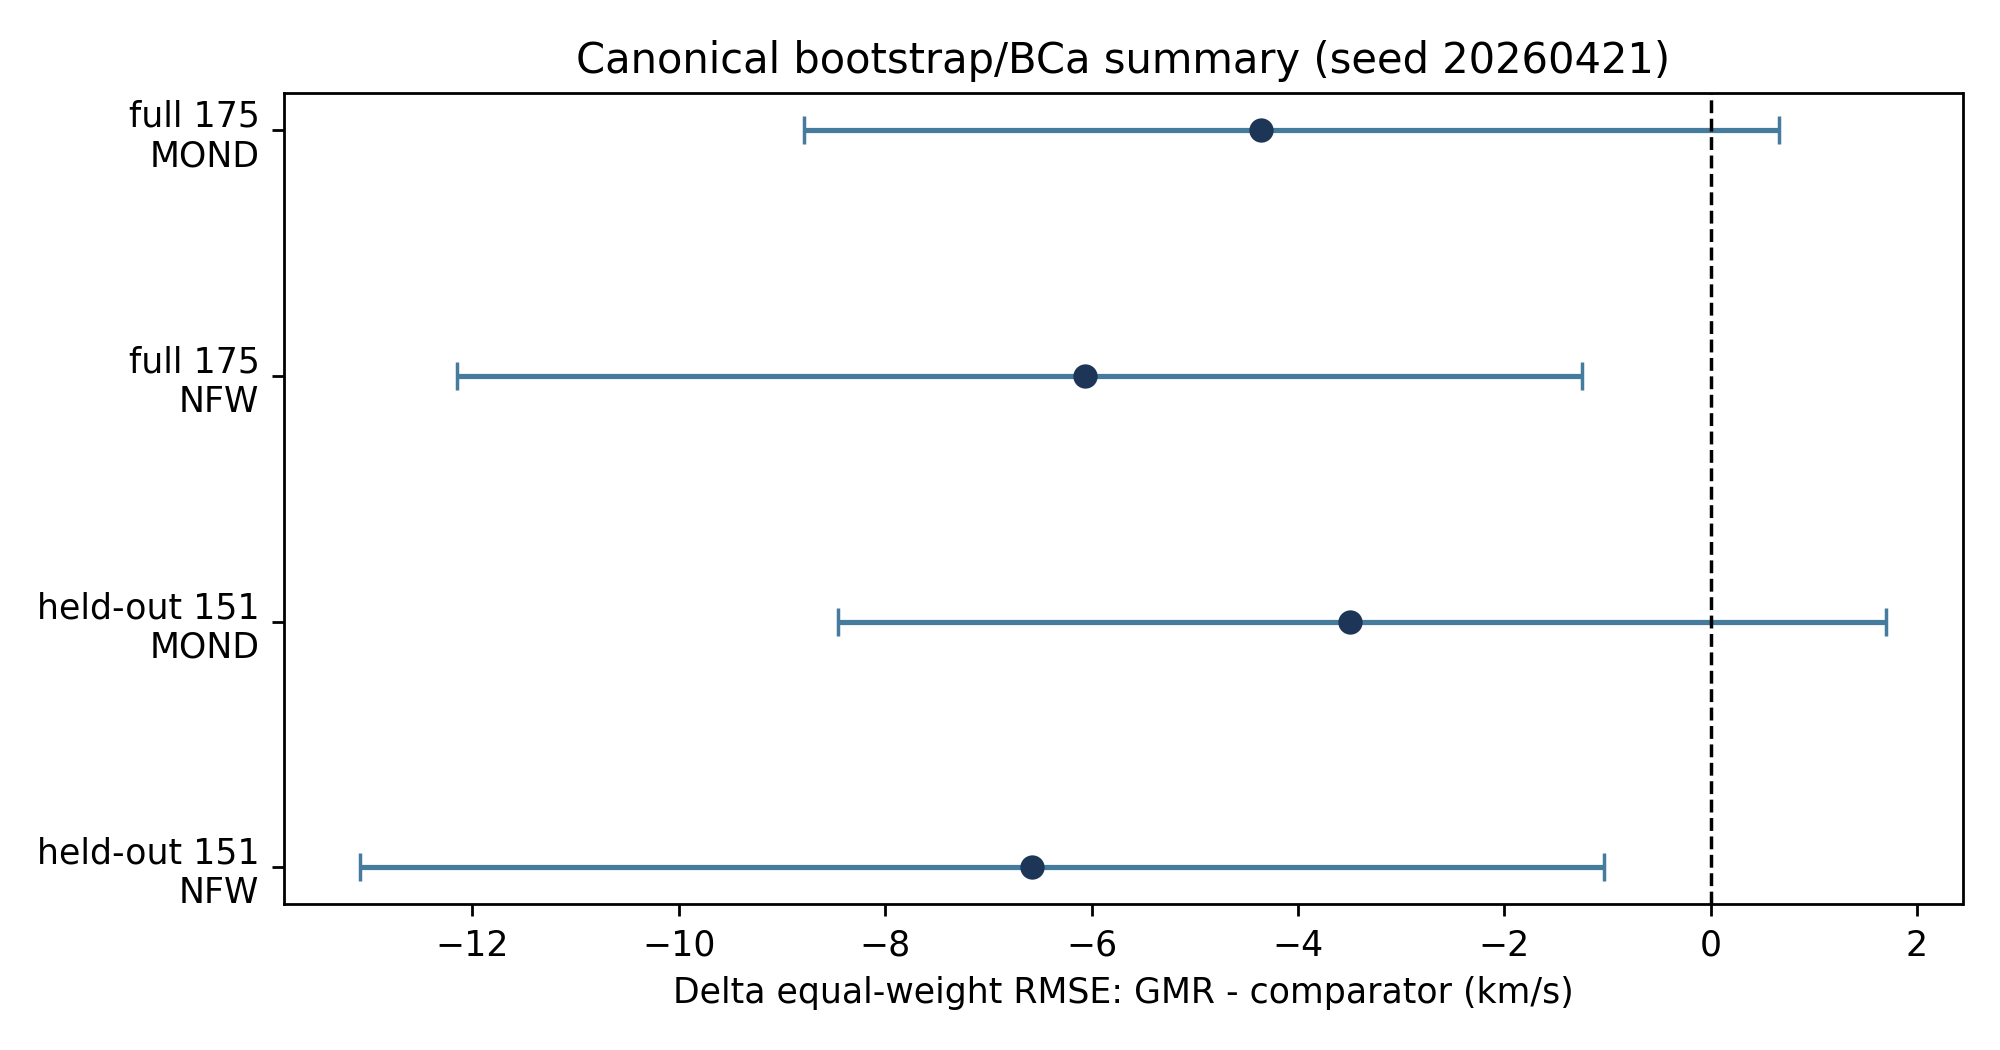
\includegraphics[width=0.92\columnwidth]{figures/V55_FIG5_bootstrap_summary.png}
\caption{Bootstrap summary for the fixed SPARC comparisons.  Several effects are descriptive rather than decisive.}
\end{figure}

\section{RAR, BTFR, and failure modes}
The RAR and BTFR checks are within-sample consistency tests.  The binned RAR curve gives a log-space RMSE of 0.0640 for fixed GMR.  It is not used as a literature-level comparison against other acceleration-law implementations.  The BTFR proxy slope is 3.687 against an observed 3.486, with broader scatter, 0.285 dex rather than 0.225 dex.  The result is slope-consistent but not scatter-matching.

\begin{figure}[t]
\centering
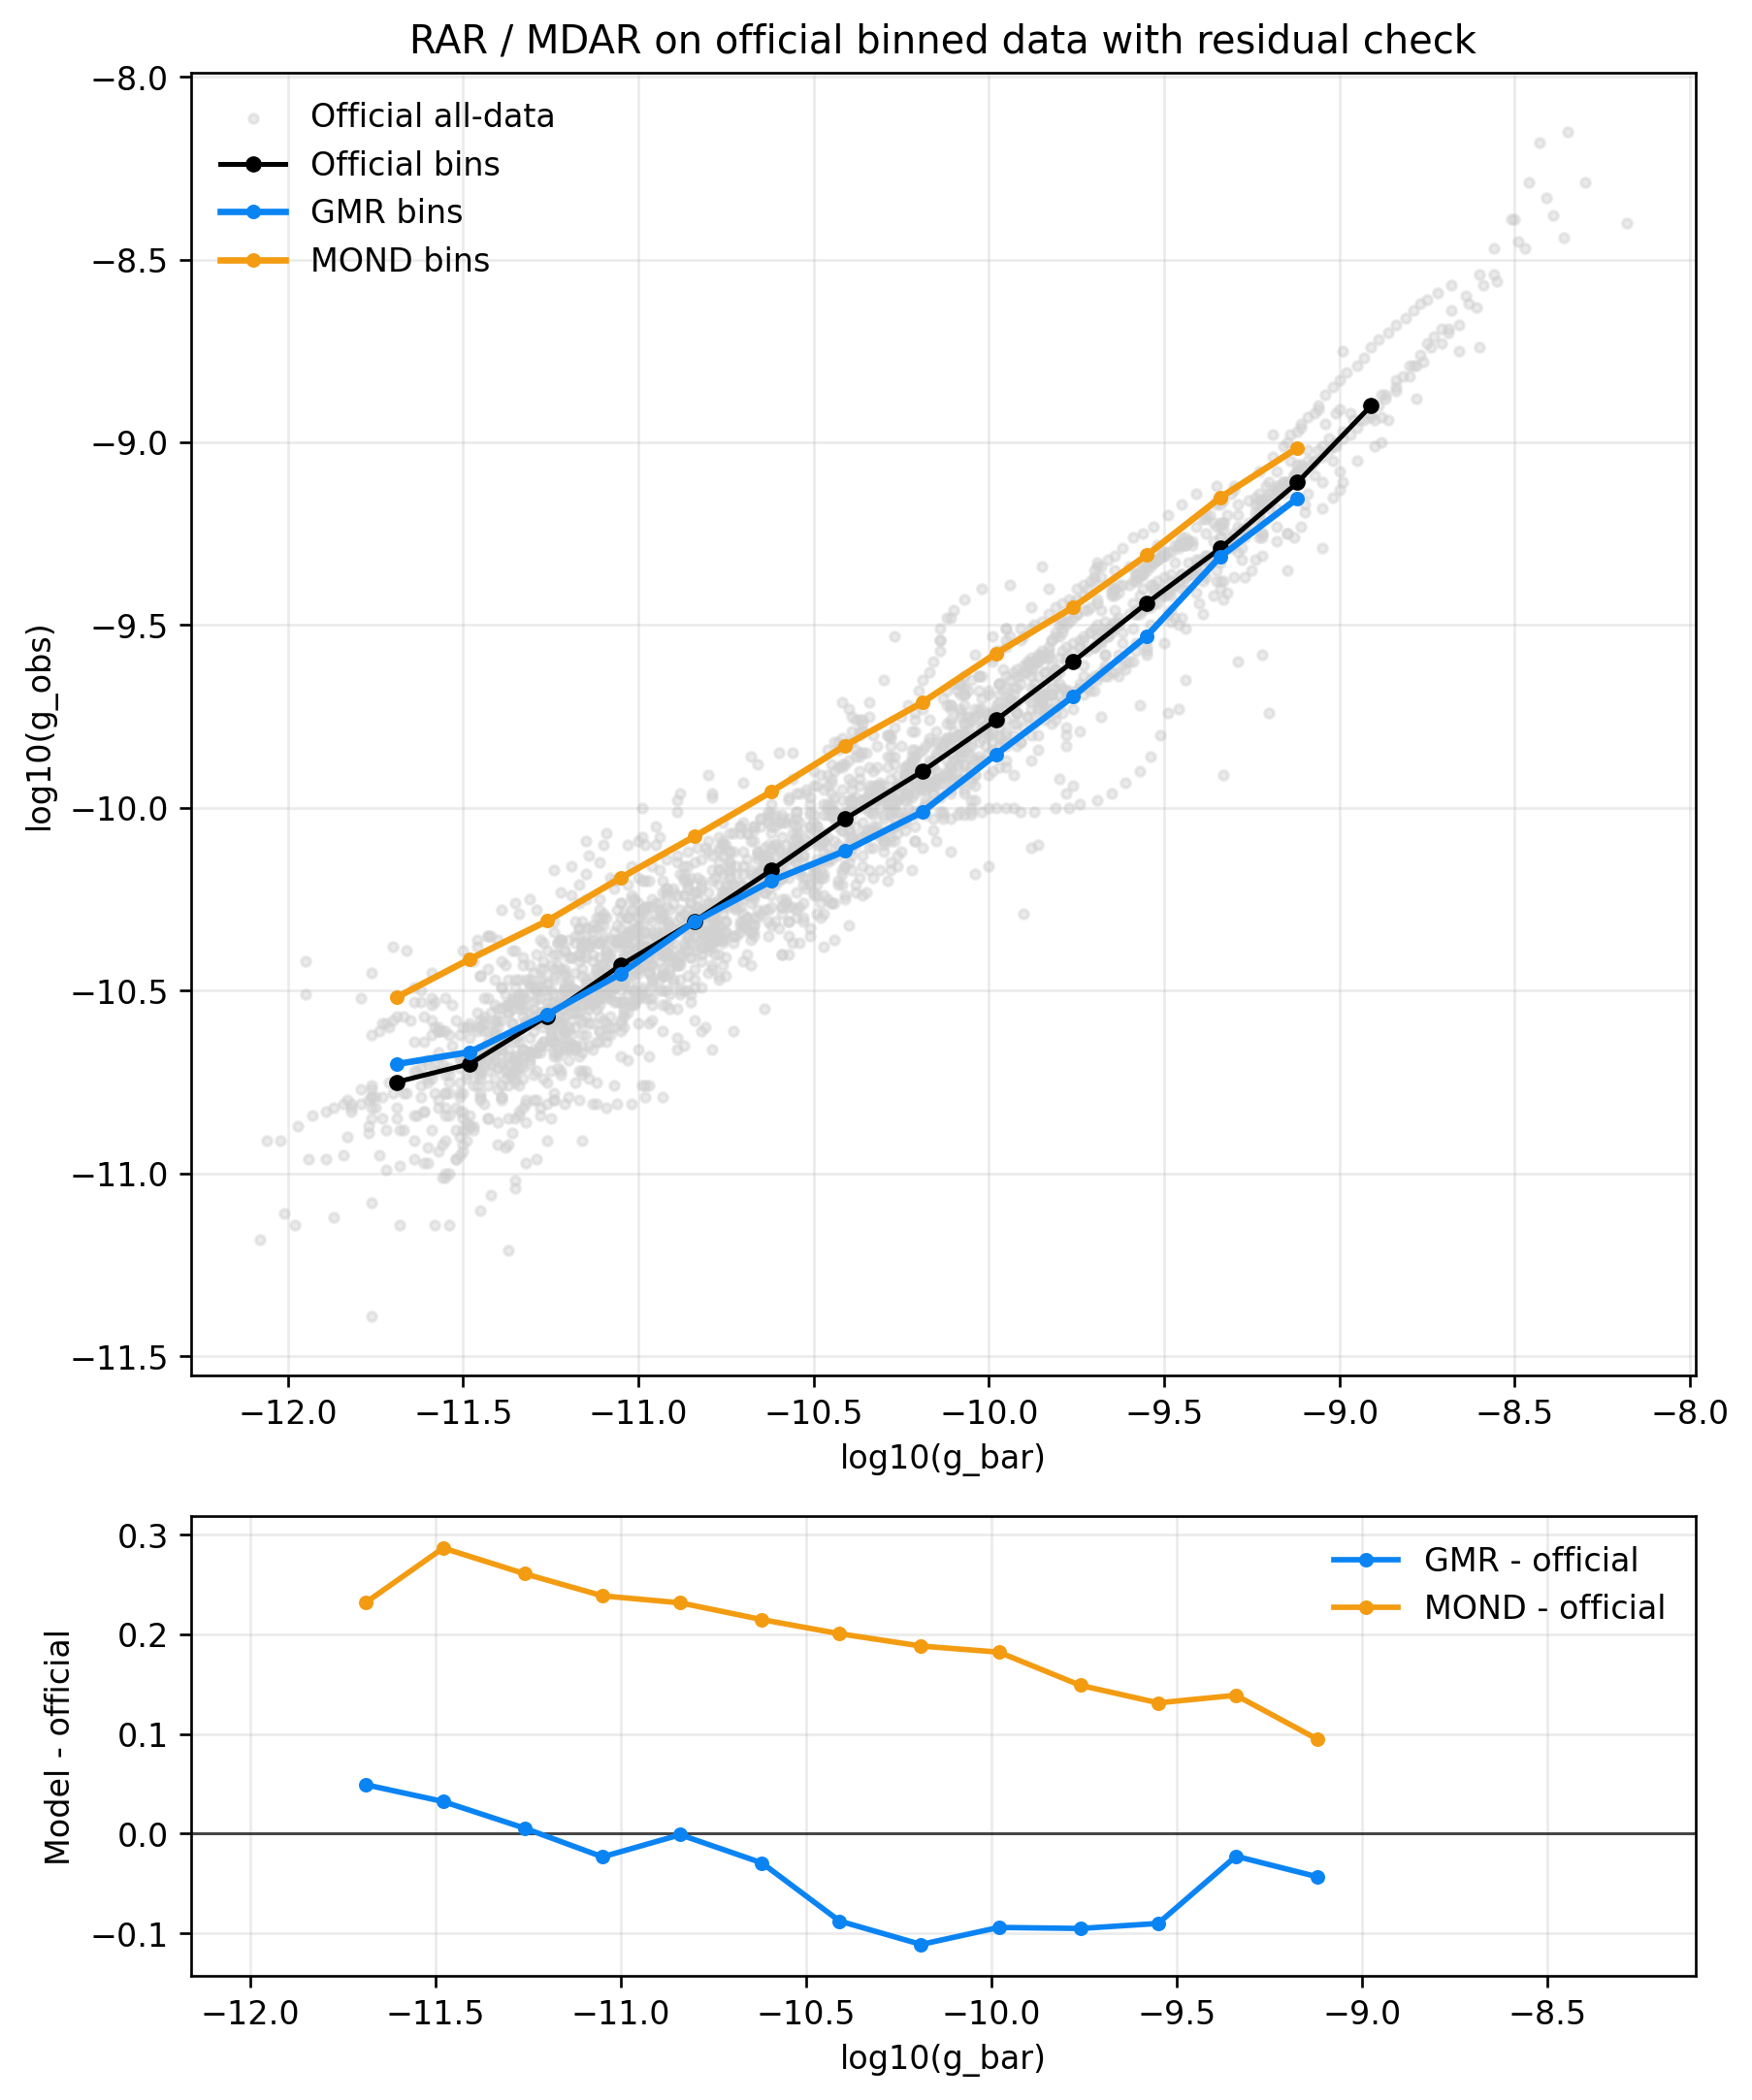
\includegraphics[width=0.92\columnwidth]{figures/V55_FIG3_RAR.png}
\caption{Binned RAR diagnostic used as a within-sample consistency check.}
\end{figure}

\begin{figure}[t]
\centering
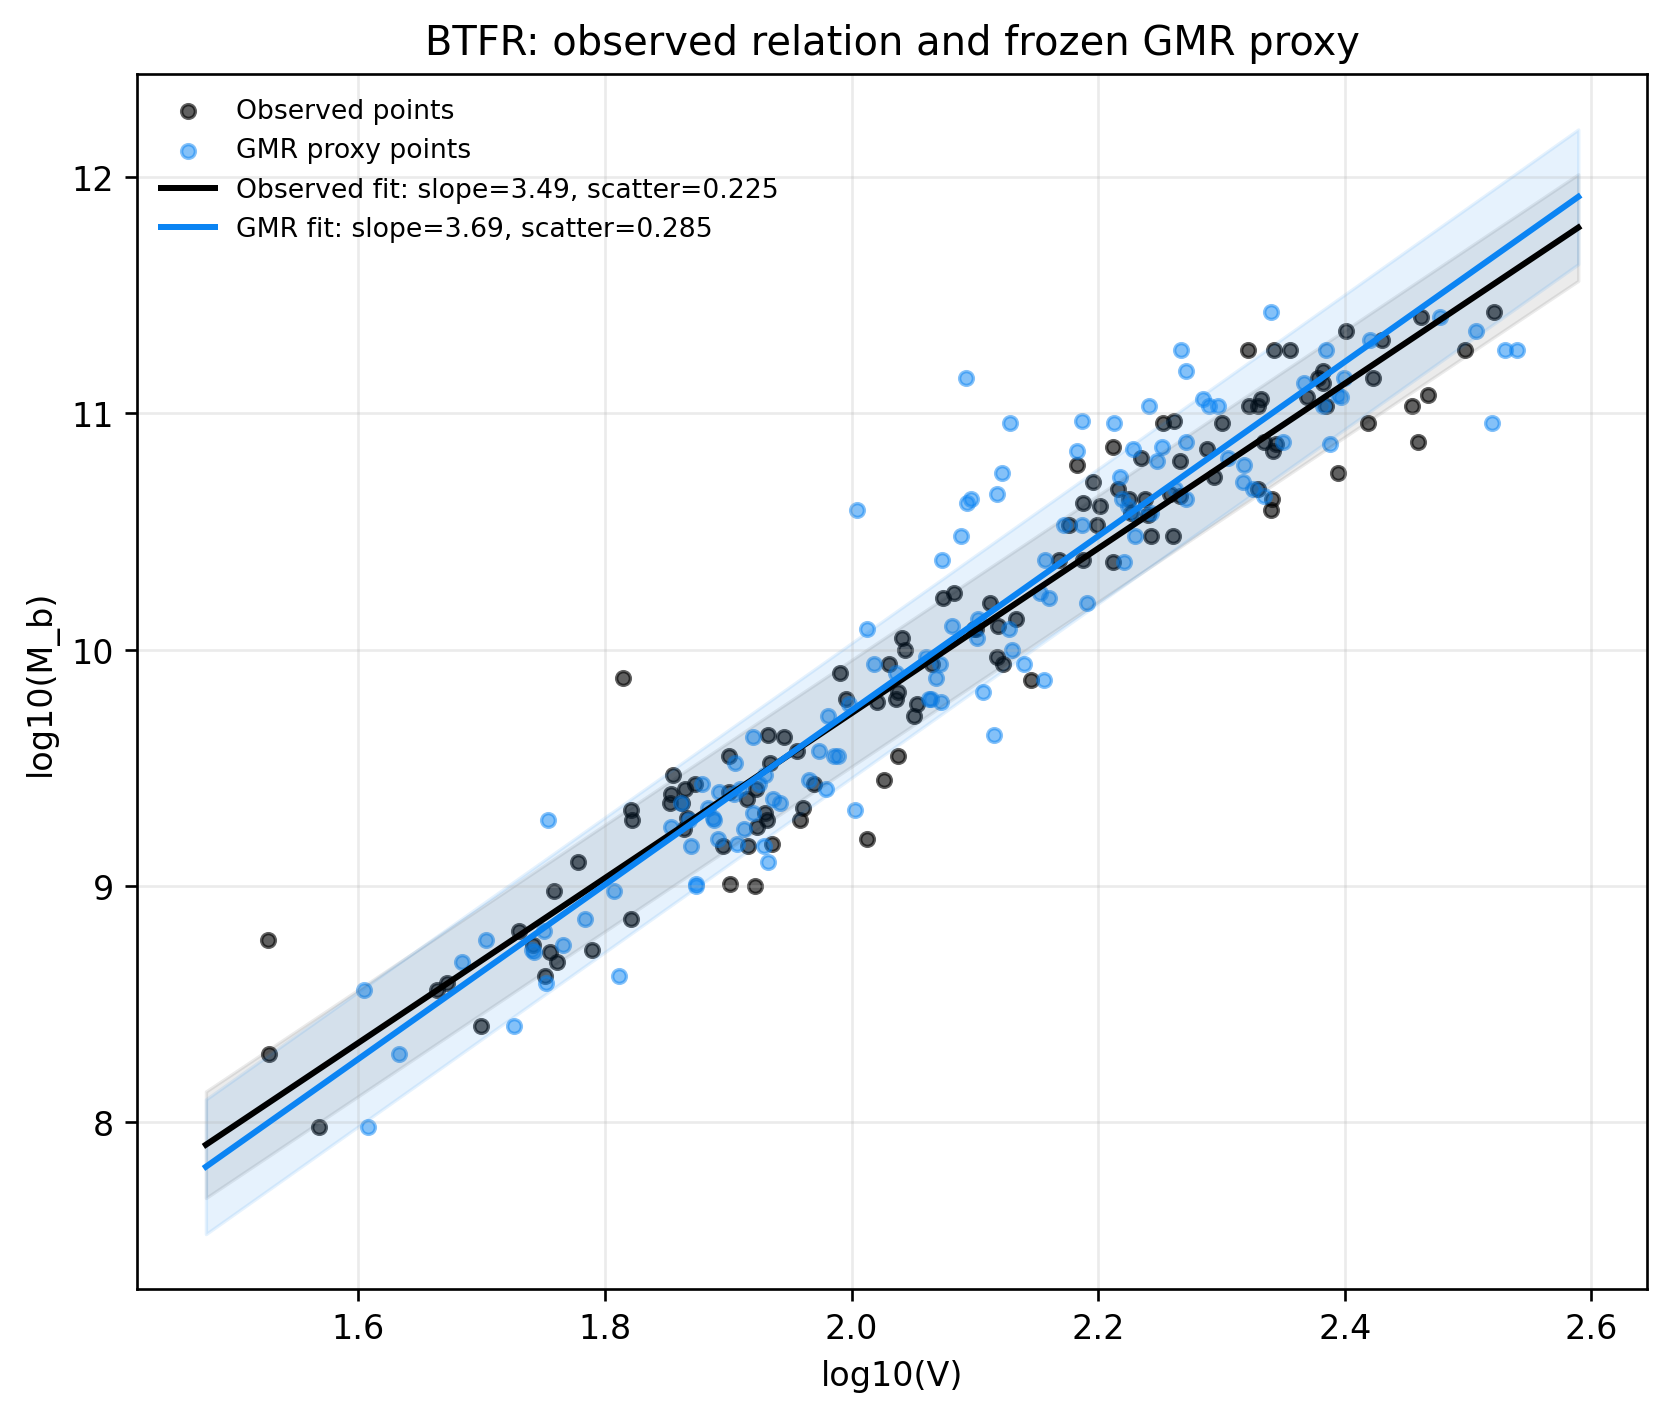
\includegraphics[width=0.92\columnwidth]{figures/V55_FIG4_BTFR.png}
\caption{BTFR diagnostic.  The proxy is slope-consistent but broader in scatter than the observed relation.}
\end{figure}

The clearest weakness of the fixed GMR prescription is the low-mass dwarf and low-surface-brightness regime.  In the low-mass-dwarf slice, GMR reaches 15.523 \kms, while reduced NFW and ISO give 6.880 and 4.478 \kms.  Ordinary disks remain difficult, and several high-leverage failures are not dwarfs, so the failure mode is principal rather than exclusive.

\begin{figure}[t]
\centering
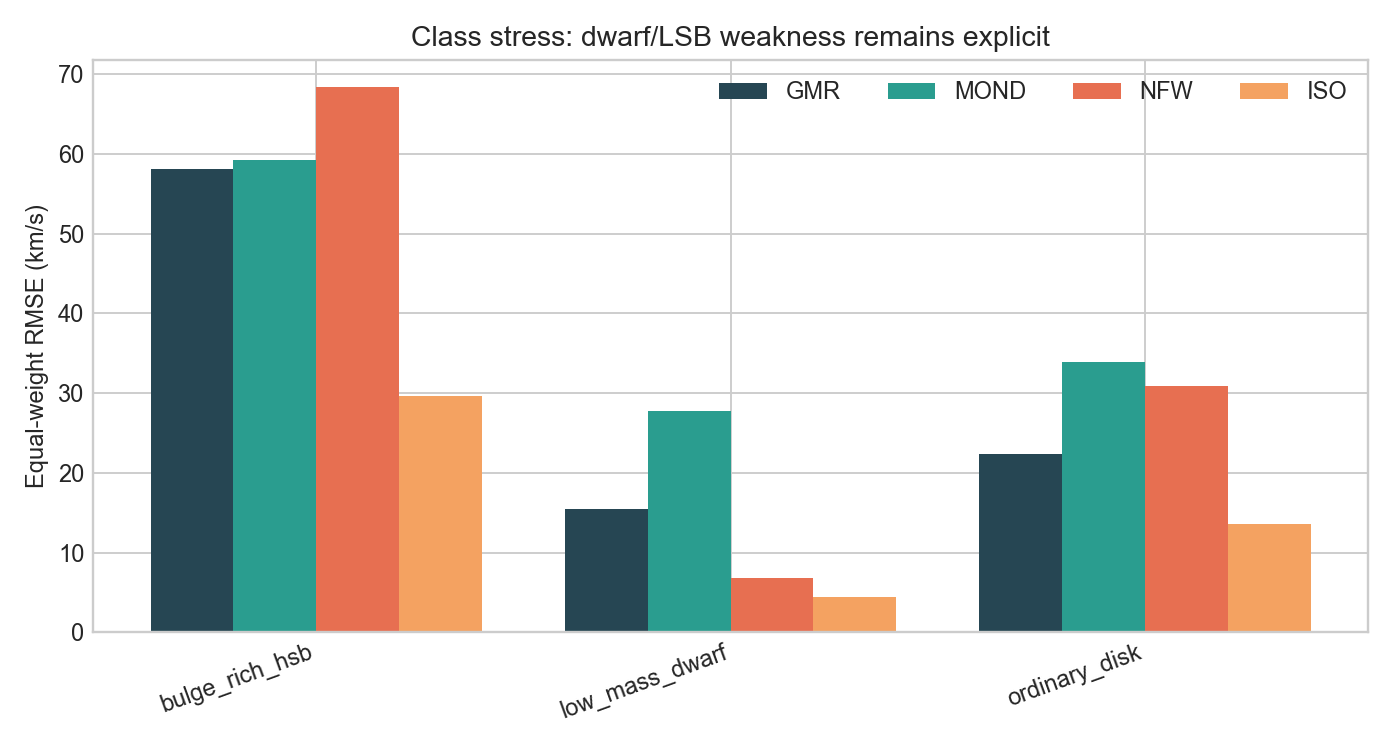
\includegraphics[width=0.92\columnwidth]{figures/R133_FIG_CLASS_STRESS.png}
\caption{Class-stress comparison.  Dwarf and low-density systems remain the sharpest empirical tension for the fixed GMR prescription.}
\end{figure}

\section{Response exponent across regimes}
The exponent comparison is mixed.  SPARC equal-weight metrics and the direct LSB component sample favor the fixed $p\simeq0.298$ branch.  LITTLE THINGS proxy tests and the validated vector-recovered subset lean toward $p=0.5$.  The rows below are fixed-branch comparisons rather than per-galaxy exponent fits: SQRT fixes $p=0.5$, FREEP fixes $p\simeq0.298$ from the internal calibration track, and the quoted objective is equal-weight per-galaxy RMSE unless stated otherwise.  Because the external evidence combines direct component tables, proxy curves, and vector-recovered components, it cannot provide a single robust posterior interval for a universal $p$.  A full per-data-set fit of $(A_p,p)$ with uncertainty propagation is needed before the exponent itself can be treated as measured separately in each regime.

\begin{table}[t]
\centering
\scriptsize
\begin{tabular}{lrrrrl}
\toprule
Data & $N$ & SQRT & FREEP & Fav. & Status\\
\midrule
SPARC full & 175 & 40.241 & 39.085 & FREEP & internal\\
SPARC holdout & 151 & 41.329 & 40.322 & FREEP & internal\\
LSB direct & 8 & 18.772 & 16.607 & FREEP & small N\\
LT proxy drop & 22 & 17.622 & 18.487 & SQRT & proxy\\
LT proxy clamp & 22 & 17.791 & 18.615 & SQRT & proxy\\
LT vector subset & 17 & 16.446 & 16.570 & SQRT & weak\\
\bottomrule
\end{tabular}
\caption{Response-exponent evidence map.  RMSE values are in \kms.  The vector-recovered LITTLE THINGS row is directional, not decisive.}
\end{table}

\begin{figure}[t]
\centering
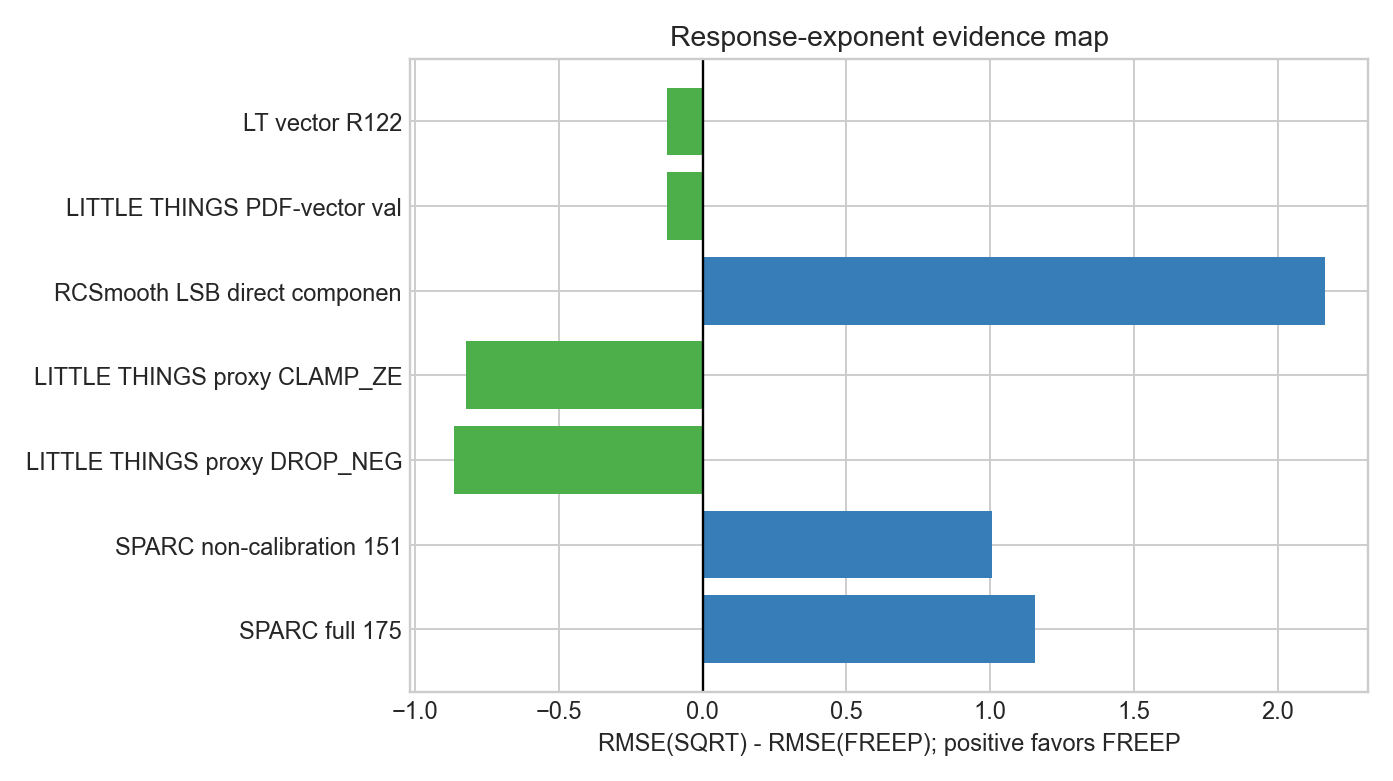
\includegraphics[width=0.92\columnwidth]{figures/R133_FIG_RESPONSE_EVIDENCE_MAP.png}
\caption{Dataset dependence of SQRT versus FREEP.  Positive values favor FREEP; negative values favor SQRT.}
\end{figure}

\begin{figure}[t]
\centering
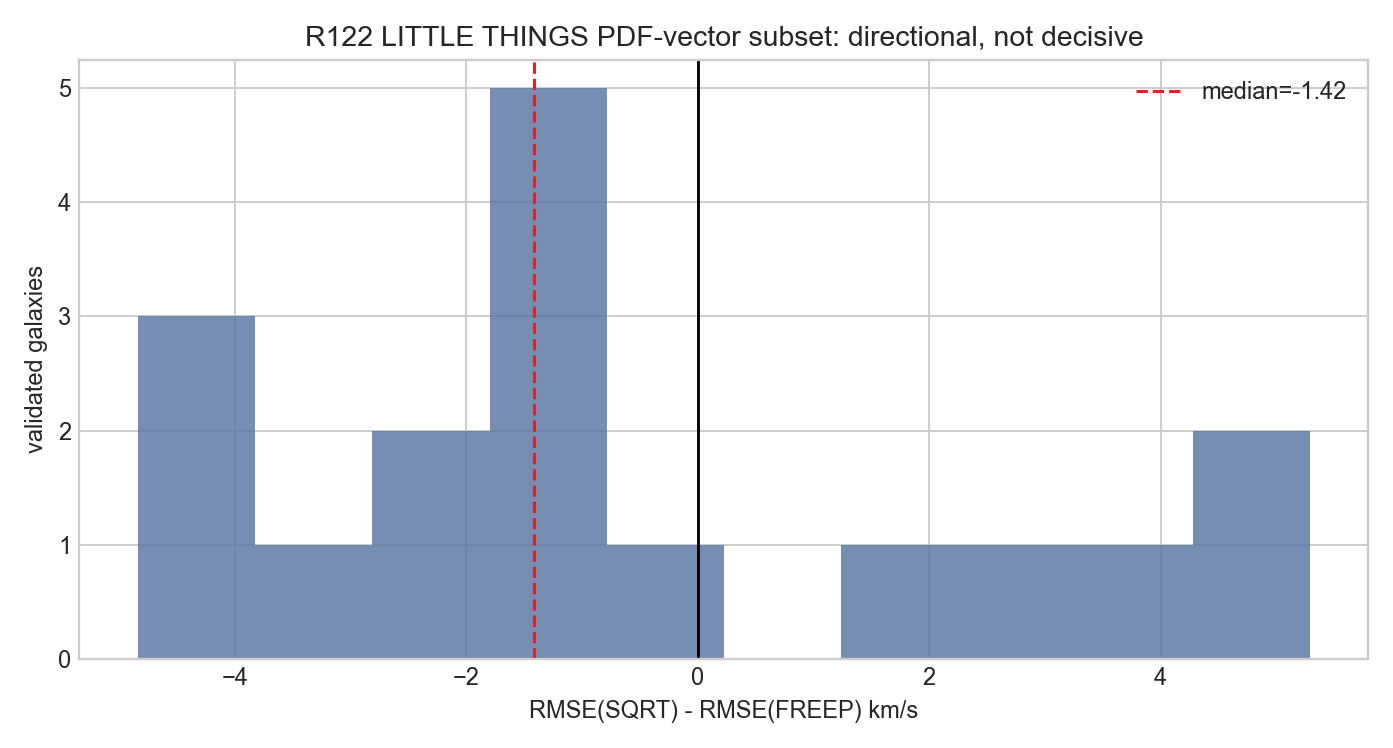
\includegraphics[width=0.92\columnwidth]{figures/R133_FIG_R122_DELTA_HISTOGRAM.png}
\caption{Per-galaxy delta distribution for the validated vector-recovered LITTLE THINGS subset.  The SQRT edge is visible but statistically weak.}
\end{figure}

The vector-recovered subset is kept conservative.  Seventeen galaxies pass validation, including fifteen GOLD and two SILVER cases.  The validation gate is independent of the SQRT/FREEP comparison: accepted cases reproduce the published reference curves well enough to be used, while rejected cases either fail that check or lack a matched dark-matter curve.  SQRT wins eleven of the seventeen, with 16.446 \kms\ versus 16.570 \kms\ for FREEP.  A paired sign test gives $p=0.332$; a galaxy-resampling bootstrap for the aggregate SQRT-minus-FREEP RMSE difference gives a 95\% interval of $[-1.76,+1.36]$ \kms\ and $P(\Delta<0)=0.609$.  This is a weak directional result.  It is consistent with the LITTLE THINGS proxy split, but it is too small and too uncertain to support a universal law.  Rejected galaxies are left outside the sample.

\section{Interpretation}
The fixed-branch comparisons suggest regime sensitivity in the projected response branch, although they stop short of measuring it as a fitted physical parameter.  The same one-parameter projection behaves differently in SPARC, direct LSB mass models, LITTLE THINGS proxy curves, and vector-recovered dwarf-galaxy components.

The channel-aware interpretation is compatible with this behavior, although the data alone cannot establish it.  A projected exponent can absorb changes in baryonic structure, gas dominance, stellar mass-to-light assumptions, response alignment, and metric weighting.  A deeper theory may still contain a more restrictive exponent, but the present evidence has not isolated one.

\section{Limitations and falsifiability}
The scope is narrower than a dark-sector solution: cluster lensing, cosmology, Solar-System screening, and a closed action are outside the present analysis.  The LITTLE THINGS component curves used here are vector-recovered from published figures; the CDS tables do not provide separate official $V_{\rm gas}/V_{\rm disk}/V_{\rm bulge}$ component curves.  The direct LSB sample is small; the SPARC free-exponent result is internal and metric-dependent; the RMSE tables lack a full galaxy-bootstrap interval for every comparator; and the summary lacks a full error-weighted $\chi^2$ reanalysis.  The cumulative $Q_{\rm enc}$ feature is also a first-order ordered radial sum, not a grid-invariant continuum functional.

The channel-aware equations are therefore a nonrelativistic phenomenological parent, not a completed relativistic gravity theory.  Any completion must satisfy post-Newtonian and Solar-System constraints, including Cassini-level bounds, and must provide screening or decoupling before the same response law is extrapolated outside galaxy rotation curves \citep{Bertotti2003,Will2014LRR,KhouryWeltman2004}.  The decisive empirical test is to obtain official or independently published direct LITTLE THINGS or THINGS component tables and repeat the no-retuning comparison.  A stronger statistical treatment should also provide the full fixed-exponent scan, error-weighted residual metrics, and bootstrap intervals for the principal RMSE comparisons.

\section{Data availability}
This preprint uses published SPARC, LITTLE THINGS, and LSB rotation-curve material.  The original survey files remain in their public archives and should be cited through the source papers.  I provide only the derived LITTLE THINGS validation table for the vector-recovered subset.  That table records which galaxies passed the recovery checks; it is not an official survey catalogue.

\section{Conclusions}
The fixed GMR prescription defines a baryonic-invariant response architecture with an explicit square-root core.  Its tested invariants do not improve the main SPARC equal-weight RMSE beyond a pure square-root control, but the cumulative state beats a local-state ablation and the comparison remains informative against baryons-only, MOND, and reduced NFW.  Cored halo baselines remain stronger overall, and the dwarf/LSB regime is the main failure mode.

The response-exponent comparison adds a second layer.  SPARC and direct LSB tests favor the fixed $p\simeq0.298$ comparator, while LITTLE THINGS proxy and vector-recovered subsets lean toward $p=0.5$ without decisive significance.  The fixed projected branches are empirically distinguishable in the present comparisons; true regime dependence of the fitted exponent remains a hypothesis requiring free-$p$ fits and propagated uncertainties.

\appendix
\section{Vector-recovered LITTLE THINGS validation subset}
The LITTLE THINGS vector-recovered check uses 17 accepted galaxies.  For each system, the accompanying table gives the validation class, the number of radial points, and the SQRT/FREEP RMSE values entering the aggregate comparison.  Nine systems fail the validation gate or lack a matched dark-matter curve and are kept outside the accepted subset.  The recovered curves show what can be read from the published figures; they are not an official LITTLE THINGS component catalogue.

\begingroup
\scriptsize
\bibliographystyle{aasjournal}
\bibliography{EMPIRICAL_RESPONSE_EXPONENTS_REFERENCES}
\endgroup
\end{document}






